\documentclass[10pt, a4paper, german]{article}
\usepackage[utf8x]{inputenc}
\usepackage{ucs} % unicode
%\usepackage[T1]{fontenc}
%\usepackage{t1enc}
%\usepackage{type1cm}
\usepackage[german]{babel}
 
\usepackage{eurosym} 
\usepackage{amsmath, amssymb}
\usepackage{graphicx}
\usepackage{natbib}
\usepackage{rotating}

\numberwithin {equation}{section}

\sloppy

\begin{document}

\begin{center}
{\large Universität Bayreuth: Philosophy \& Economics, SoSe 2009}
\end{center}
\vspace{0.4em}
\begin{center}
{\huge {\bf Lösung} zur Klausur: Grundlagen des Entscheidens I}
\end{center}
\vspace{0.0em}
\begin{center}
Datum: 20. August 2009\\
Dozent: Eckhart Arnold
\end{center}

\begin{quote}
  {\em Zum Besseren Verständnis habe ich die Lösungen zu den Aufgaben mit
  ausführlichen Erklärungen versehen. In der Klausur war das natürlich
  nicht gefordert. Es reicht das richtige Ergebnis bzw. die richtige
  Rechnung.}
\end{quote}

\section{Aufgabe: Bayes und Entscheidungsbäume}

% Eine Ölfirma möchte in der Nordsee eine Bohrinsel (Kosten: 10 Mio Euro)
% errichten, um Öl zu fördern. 
% Die Wahrscheinlichkeit, innerhalb dieses Gebiets auf Öl zu stoßen, beträgt 60\%.
% Im Erfolgsfall rechnet die Firma mit Einnahmen von 50 Mio Euro. 
% 
% Ein Geologe bietet der Firma für 1 Mio Euro für die Durchführung einer Expertise
% an. Ist tatsächlich Öl vorhanden, so wird dies durch die Expertise mit
% 95\%-iger Sicherheit festgestellt werden. Ist kein Öl vorhanden, so wird dies
% durch die Expertise mit 85\%-iger Sicherheit festgestellt.
% 
% \begin{enumerate}
%   \item Angenommen, die Expertise wird durchgeführt und fällt positiv aus. Wie
%   groß ist die Wahrscheinlichkeit, dass tatsächlich Öl vorhanden ist?
%   \item Angenommen, die Expertise fällt negativ aus. Wie groß ist die
%   Wahrscheinlichkeit, dass trotzdem Öl vorhanden ist?
% %   \item Wie groß ist die Wahrscheinlichkeit, dass die Expertise positiv
% %   ausfällt?
%   \item Stellen Sie den Entscheidungsbaum auf und beantworten Sie die Frage, ob
%   die Firma die Expertise durchführen sollte oder nicht.
% %   \item Angesichts der Tatsache, dass die Entscheidung für den Bau einer
% %   Ölplattform bei einem positiven Erwartungswert von
% %   $0,6 \cdot 40 Mio + 0.4 \cdot -10 Mio = 20 Mio Euro$ auch ohne Expertise
% %   kaum zweifelhaft sein dürfte, argumentiert jemand, dass die Durchführung einer Expertise 
% %   überflüssig ist. Stimmt das Argument? Wenn ja, warum? Wenn nein, warum nicht?
% \end{enumerate}

Im Folgenden sei mit ``$o$'' das Ereignis bezeichnet, dass Öl vorhanden ist und
mit ``$\neg o$'' das Ereignis, dass kein Öl vorhanden ist. Weiterhin soll
``$e$'' dafür stehen, dass die Expertise positiv ausfällt, und ``$\neg e$''
dafür, dass sie negativ ausfällt. (Beispiel: Die bedingte Wahrscheinlichkeit,
dafür dass Öl vorhanden ist, wenn die Expertise negativ ausgefallen ist, wird
mit ``$P(o|\neg e)$'' bezeichnet.) 

\vspace{0.3cm}

\setlength{\parindent}{0cm}
In der Aufgabe angegeben sind
die folgenden Wahrscheinlichkeiten:

\vspace{0.1cm}

\begin{tabular}{lll}
$P(o)$&$   = 0.6$  & Basisrate \\
$P(e|o)$&$ = 0.95$ & Positiv-Positiv-Rate \\
$P(\neg e| \neg o)$&$ = 0.85$ & Negativ-Negativ-Rate \\ 
\end{tabular}

\vspace{0.3cm}

Unmittelbar daraus ableiten kann man die entsprechenden inversen
Wahrscheinlichkeiten:

\vspace{0.1cm}

\begin{tabular}{lll}
$P(\neg o)$&$ = 0.4$    & Wahrscheinlichkeit, dass kein Öl vorhanden ist \\
$P(\neg e|o)$&$ = 0.05$ & Negativ-Positiv-Rate \\
$P(e|\neg o)$&$ = 0.15$ & Positiv-Negativ-Rate \\
\end{tabular}

\vspace{0.3cm}

Begnötigt werden zur Lösung des Entscheidungsproblems noch diese
Wahrscheinlichkeiten:

\vspace{0.1cm}

\begin{tabular}{lll}
$P(o|e)$&$ ={ } ?$  & Teilaufgabe 1 \\
$P(o|\neg e)$&$ ={ } ?$ & Teilaufgabe 2 \\
$P(e)$&$ ={ } ?$ & Wahrscheinlichkeit, dass die Expertise positiv ausfällt
\\
\end{tabular}

\subsection{Lösung der 1. Teilaufgabe (Bayes)}

Lösung durch einfaches Einsetzen in die Bayes'sche Formel.

\begin{eqnarray*}
P(o|e) & = & \frac{P(e|o)P(o)}{P(e|o)P(o) + P(e|\neg o)P(\neg o)} \\
       & = & \frac{0,95\cdot 0,6}{0,95\cdot 0,6 + 0,15\cdot 0,4} = 0,905 
\end{eqnarray*}

Die Wahrscheinlichkeit, mit der Öl vorhanden ist, wenn die Expertise positiv
ausfällt, beträgt: 90,5\%.

\subsection{Lösung der 2. Teilaufgabe (Bayes)}

Lösung durch Einsetzen in die Bayes'sche Formel. Dabei ist zu beachten, dass
an einigen Stellen die inversen Wahrscheinlichkeiten verwendet werden müssen.

\begin{eqnarray*}
P(o|\neg e) & = & \frac{P(\neg e|o)P(o)}{P(\neg e|o)P(o) + P(\neg e|\neg
o)P(\neg o)} \\ & = & \frac{0,05\cdot 0,6}{0,05\cdot 0,6 + 0,85\cdot 0,4} 
= 0,081
\end{eqnarray*}

% Alternative Lösung:

% \begin{eqnarray*}
% P(o|\neg e) = 1 - P(\neg o|\neg e)& = & 
% 1-\frac{P(\neg e|\neg o)P(\neg o)}{P(\neg e|\neg o)P(\neg o) 
% + P(\neg e|o)P(o)} \\ & = & 1-\frac{0,85\cdot 0,4}{0,85\cdot 0,4 +
% 0,05\cdot 0,6} \\ & = & 1 - 0,919 = 0,081
% \end{eqnarray*}

Die Wahrscheinlichkeit, mit der doch Öl vorhanden ist, wenn die Expertise
negativ ausfällt, beträgt 8,1\%.

\subsection{Lösung der 3.Teilaufgabe (Entscheidungsbaum)}

Vor der Aufstellung des Entscheidungsbaums ist zunächst die Wahrscheinlichkeit
dafür zu berechnen, dass die Expertise positiv ausfällt. Auf Grund der
Fehlerraten der Expertise ist diese Wahrscheinlichkeit {\em nicht} identisch
mit der Wahrscheinlichkeit, mit der Öl vorhanden ist! Berücksichtigt man, dass
die Expertise immer dann positiv ausfällt, wenn entweder a) Öl vorhanden ist
und die Expertise dies richtig anzeigt, oder b) kein Öl vorhanden ist, aber die
Expertise trotzdem das Vorhandensein von Öl anzeigt, dann berechnet sich die
die Wahrscheinlichkeit so:

\vspace{0.2cm}
$P(e) = P(e|o)\cdot P(o) + P(e|\neg o)\cdot P(\neg o) = 
0,95\cdot 0,6 + 0,15\cdot 0,4 = 0,626$

\vspace{0.2cm}
Die Wahrscheinlichkeit, dass die Expertise (bei der gegebenen Basisrate und
gegebenen Fehlerraten) positiv ausfällt, beträgt also 62,6\%.

\vspace{0.2cm}
An den Enden (den ``Blättern'') des Entscheidungsbaums sind die Netto-Kosten
(bzw. der Netto-Ertrag) des jeweiligen Ergebnisses einzutragen. Bei der
Auflösung des Entscheidungsbaums sind an den Zufallsknoten die 
Erwartungswerte zu berechnen. Im Einzelnen sind das folgende Erwartungswerte:

\begin{enumerate}

\item Der Erwartungswert für den Bau einer Ölplattform, wenn die
  Expertise positiv ausgefallen ist:
  $EW_1 = 0,905\cdot 39 + 0,095\cdot -11 = 34,25 \quad \mbox{Mio €}$

\item Der Erwartungswert für den Bau einer Ölplattform, wenn die
  Expertise negativ ausgefallen ist:
  $EW_2 = 0,081\cdot 39 + 0,919\cdot -11 = -6,95 \quad \mbox{Mio €}$

\item Der Erwartungswert bei der Durchführung einer Expertise:\\
  $EW_3 = 0,626\cdot 34,25 + 0,374\cdot -1 = 21,0665 \quad \mbox{Mio €}$

\item Der Erwartungswert für den Bau einer Ölplattform, wenn keine
  Expertise durchgeführt wird:
  $EW_4 = 0,6\cdot 40 + 0,4\cdot -10 = 20 \quad \mbox{Mio €}$

\end{enumerate}

Da der Erwartungswert bei der Durchführung einer Expertise ($EW_3 =
21,0665$ Mio €) höher ausfällt, als wenn keine Expertise durchgeführt
wird ($EW_4 = 20$ Mio €), sollte die Expertise durchgeführt werden.


\begin{sidewaysfigure}
\begin{center}
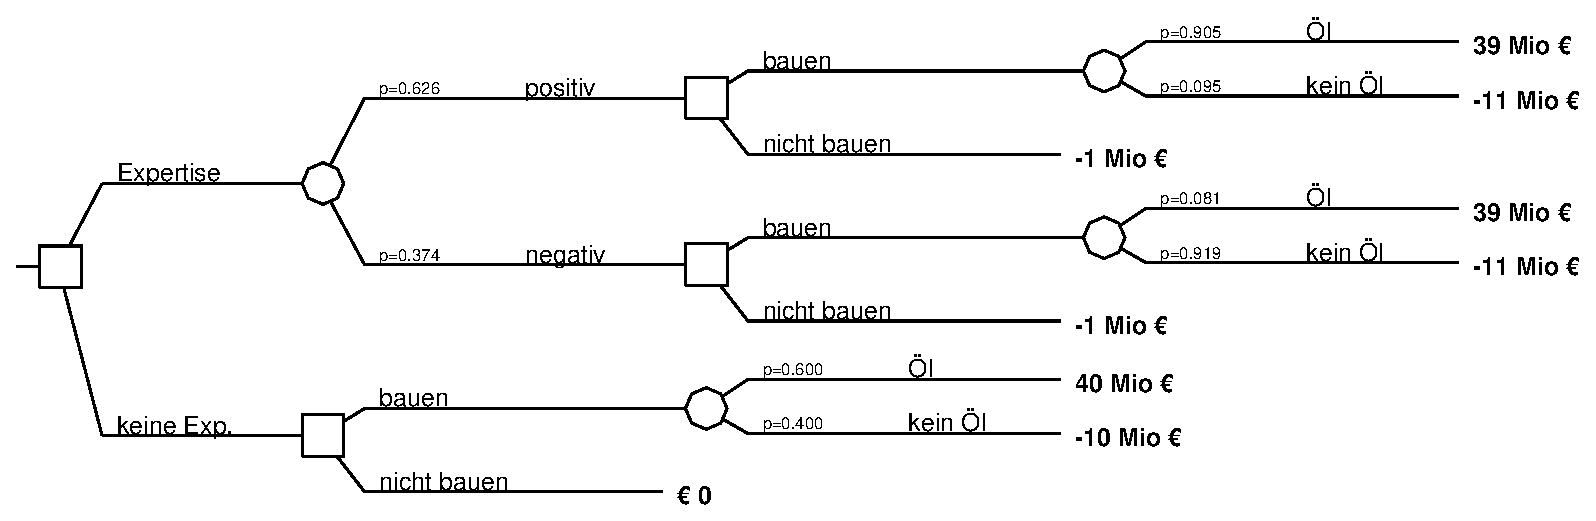
\includegraphics[width=22cm]{Grafiken/Klausur_2009.eps}
\caption{Der Entscheidungsbaum zur 1. Aufgabe.}
\end{center}
\end{sidewaysfigure}


\section{Aufgabe: Wahlverfahren}

% Bei der Abstimmung über drei Kandidaten $A, B, C$ für ein bestimmtes Amt stehen
% folgende drei Abstimmungsverfahren zur Auswahl: a) {\em Stimme für Einen}:
% Jeder Wähler schreibt seinen bevorzugten Kandidaten auf einen
% Zettel; der Kandidat mit den meisten Stimmen gewinnt. b) {\em Stimme für Zwei}:
% Jeder Wähler schreibt seine zwei bevorzugten Kandidaten auf einen Zettel; der
% mit den meisten Stimmen bzw. Nennungen gewinnt. c) {\em Borda-Zählung}: Jeder
% vergibt Punkte für die Kandidaten, und zwar 2 Punkte für den am meisten
% bevorzugten Kandidaten, 1 Punkt für den mittleren und 0 Punkte für den am
% wenigsten geschätzten Kandidaten; der Kandidat mit den meisten Punkten gewinnt.

% \begin{enumerate}
%   \item Finden Sie ein Präferenzprofil, bei dem nach dem Abstimmungsverfahren
%   a) {\em Stimme für Einen} ein anderer Kandidat gewinnt als nach dem
%   Abstimmungsverfahren b) {\em Stimme für Zwei}.
%   \item Finden Sie ein Präferenzprofil, bei dem nach jedem der drei
%   Abstimmungsverfahren ein anderer Kandidat gewinnt.
% \end{enumerate}

% Es sollen immer genau drei Kandidaten vorkommen. Die Anzahl der Wähler kann
% frei gewählt werden.

\subsection{Lösung der 1. Teilaufgabe}

\begin{center}
\begin{tabular}{c|c}
Präferenzen & Anzahl der Wähler \\
der Wähler  & mit diesen Präferenzen \\
\cline{1-2}
 & \\ 
$A \succ B \succ C$ & 2 \\
$B \succ C \succ A$ & 1 \\
\end{tabular}
\end{center}

Bei dieser Verteilung von Präferenzen auf zwei Wählergruppen gewinnt A
bei dem Verfahren ``Stimme für Einen'' mit 2 zu 1 Stimmen. Bei dem
Verfahren ``Stimme für Zwei'' gewinnt B aber mit 3 zu 2 Stimmen!

\vspace{0.2cm} Wie auch bei der folgenden Aufgabe ist die Lösung nicht
eindeutig, sondern es existieren viele Andere Lösungen.

\subsection{Lösung der 2. Teilaufgabe}

\subsubsection{Lösung durch Raten}

Eine der einfachsten Lösungen lautet:

\begin{center}
\begin{tabular}{c|c}
Präferenzen & Anzahl der Wähler \\
der Wähler  & mit diesen Präferenzen \\
\cline{1-2}
 & \\ 
$A \succ B \succ C$ & $6$  \\
$A \succ C \succ A$ & $5$  \\
$C \succ B \succ A$ & $10$ \\
\end{tabular}

\vspace{0.5cm}
\begin{tabular}{c|c|ccc|c|ccc|c|c}
\multicolumn{3}{c}{Eine St.} & & \multicolumn{3}{c}{Zwei St.} & & \multicolumn{3}{c}{Borda} \\
A       & B & C              & &  A & B        & C            & & A  & B  & C \\
\cline{1-3} \cline{5-7} \cline{9-11} % & & & & & & & & & & \\

{\bf 11} & 0 & 10            & & 11 & {\bf 16} & 10           & & 22 & 16 & {\bf 25} \\
\end{tabular}
\end{center}

\vspace{0.2cm} Am besten lässt sich eine Lösung erraten, wenn
man gleich mit etwas größeren Zahlen ansetzt. 
Weitere mögliche Lösungen sind u.a.:
$(5,3,0,0,7,0)$; $(11,0,0,0,3,9)$; $(3,4,0,6,0,0)$;
$(1,0,4,0,3,2)$; $(4,5,0,8,3,0)$; $(10,2,0,1,11,0)$; $(11,6,0,9,0,15)$;
$(10,5,0,8,0,14)$; $(101,5,0,3,0,103)$; $(6,2,0,4,2,5)$; $(5,2,0,3,1,5)$; $(12,2,0,7,6,7)$ 
Das sind natürlich nur Beispiele. Die Lösungmenge als solches ist unendlich
groß.

\subsubsection{Lösung mit Vorüberlegungen}

Eine Lösung ist durch reines Ausprobieren nicht unbedingt
leicht zu finden. Die Suche nach der richtigen Lösung wird aber stark
vereinfacht, wenn man zunächst einige Vorüberlegungen
anstellt. Zunächst einmal lässt sich das Problem mathematisch als die
Suche nach den Werten von 6 Unbekannten $x_1, ..., x_6$ auffassen, die
den in der Aufgabe genannten Bedingungen genügen müssen:

\begin{center}
\begin{tabular}{c|c}
Präferenzen & Anzahl der Wähler \\
der Wähler  & mit diesen Präferenzen \\
\cline{1-2}
 & \\ 
$A \succ B \succ C$ & $x_1$ \\
$A \succ C \succ A$ & $x_2$ \\
$B \succ A \succ C$ & $x_3$ \\
$B \succ C \succ A$ & $x_4$ \\
$C \succ A \succ B$ & $x_5$ \\
$C \succ B \succ A$ & $x_6$ \\
\end{tabular}
\end{center}

Nun kann man z.B. folgende Überlegungen anstellen:

\begin{enumerate}
\item Angenommen $A$ soll Gewinner nach dem Verfahren ``Eine Stimme''
  sein und $C$ nach der Borda-Zählung. Dann sollte, da die
  Borda-Zählung vergleichsweise sensitiv auf die Höchsplatzierung
  reagiert, die Häufigkeit, mit der $A$ höchstplatziert wird, nur
  möglichst geringfügig größer sein als die Häufigkeit, mit der $C$
  in den Wählerpräferenzen höchstplaziert wird. Man kann also annehmen:
  \[ x_1 + x_2 = x_5 + x_6 + 1\]

\item Eine Möglichkeit, den Nachteil von $C$ bei der Borda-Zählung
  auszugleichen, besteht darin, diejenige Wählerpräferenz zu erhöhen,
  bei der $C$ an zweiter Stelle und $A$ an dritter Stelle steht. Da
  $C$ nur an zweiter Stelle vorkommt, kann der Nachteil nur
  ausgeglichen werden, wenn diese Präferenz von mehr als zwei Wählern
  vertreten wird, also wenn:
  \[ x_4 \geq 3 \]

\item Um zu erreichen, dass $B$ nach dem Verfahren ``Zwei Stimmen''
  gewinnt, bietet es sich an, gleichmäßig $x_1$ und $x_6$ zu erhöhen,
  da mit jeder gleichmäßigen Erhöung das ``Zwei Stimmen''-Ergebnis
  von $B$ um zwei Punkte vorrückt, während $A$ und $C$ nur um einen
  Punkt vorrücken. (Die (relative) Borda-Platzierung bleibt davon
  unberührt.) Man kann also davon ausgehen, dass jeweils:
  \[ x_1 \gg x_2 \qquad \mbox{und} \qquad x_6 \gg x_5 \]

\item Solange aber $x_2 = 0$ und $x_5 = 0$ genießt $B$ wegen $x_4 \geq 3$
  nach der Borda-Zählung noch einen Vorsprung vor $C$ von mind. 3
  Punkten. Daher müssen $x_2$ und $x_5$ mindestens so groß gesetzt
  werden, dass sie diesen Vorsprung gerade eben ausgleichen,
  d.h. beispielsweise $x_2=2$ und $x_5=1$. Allgemein muss gelten:
  \[ 2x_5 + x_2 > x_4/2 \] 
\end{enumerate}

\vspace{0.2cm}
Setzt man nun probehalber $x_4 = 3$ (wegen der 2. Überlegung), und
$x_2$ und $x_5$ auf kleine Werte (wegen der 4. Überlegung) sowie $x_1$
und $x_6$ auf merklich größere Werte (wg. der 3. Überlegung) und
berücksichtigt, dass entweder $x_6 < x_1$ oder $x_5 < x_2$ (wegen der
1. Überlegung), dann kommt man einigermaßen schnell zu einer Lösung wie:
$x_1=10, x_2=2, x_3=0, x_4=3, x_5=1, x_6=10$


\subsubsection{Allgemeiner Lösungsansatz}

Für Interessierte sei noch darauf hingewiesen, dass es auch einen
systematischen Ansatz zur Lösung des Problems gibt, der sich sogar auf
beliebige Wahlverfahren (vom selben Typ wie die Borda-Zählung)
verallgemeinern lässt. Der Ansatz sei hier nur angedeutet:

\vspace{0.2cm}
Wenn $A$ Gewinner bei dem Wahlverfahren ``Eine Stimme'' sein soll,
dann muss die Gesamtstimmenzahl von $A$ größer sein als die von $B$
und auch größer als die von $C$.  Mathematisch lässt sich das durch
die beiden Ungleichungen ausdrücken:

\vspace{0.2cm}
\begin{math}
\mbox{U1:} \qquad x_1 + x_2 > x_3 + x_4 \\
\mbox{U2:} \qquad x_1 + x_2 > x_5 + x_6 
\end{math}

\vspace{0.2cm}
Wenn $B$ Gewinner bei dem Wahlverfahren ``Zwei Stimmen'' sein soll, 
dann lässt sich das mathematisch ebenfalls durch zwei Ungleichungen ausdrücken:

\vspace{0.2cm}
\begin{math}
\mbox{U3:} \qquad x_4 + x_6 > x_2 + x_5 \\
\mbox{U4:} \qquad x_1 + x_3 > x_2 + x_5 
\end{math}

\vspace{0.2cm}
Dass $C$ nach der Borda-Zählung gewinnt, bedeutet mathematisch:

\vspace{0.2cm}
\begin{math}
\mbox{U5:} \qquad x_4 + x_5 + 2x_6 > 2x_1 + x_2 + x_3 \\
\mbox{U6:} \qquad x_2 + 2x_5 + x_6 > x_1 + 2x_3 + x_4 
\end{math}

\vspace{0.2cm}

Das Problem ist damit auf ein System von Ungleichungen zurückgeführt,
zu dessen Lösung man dann Verfahren der Linearen Algebra bzw. der
angewandten Mathematik heran ziehen würde. In der Klausur war das
natürlich nicht gefordert. 

In diesem Fall ist das Ungleichungssystem übrigens hochgradig unterbestimmt.
Wenn man eine Lösung durch herumprobieren finden will, empfiehlt es sich daher
zunächst einfach ein par Variablen konstant (am besten auf 0) zu setzen, und
für die verbleibenden die Ungleichungen aufzulösen. (Falls das nicht auf
Anhieb geht, wählt man andere Variablen, die man konstant setzt.)



\section{Aufgabe Lotterien}

% Sei ${\cal G}$ eine Menge von Grundgütern auf der eine Menge ${\cal L}$ von
% Lotterien der Form $L(a, x, y)$ definiert ist, wobei $0 \leq a \leq 1$ und $x$
% und $y$ jeweils entweder Gründgüter oder wiederum Lotterien sind. Sei weiterhin
% $B \in {\cal G}$ ein bestes Gut aus der Menge der Grundgüter, d.h. es gelte
% für jedes Grundgut $x \in {\cal G}$, dass $B \succeq x$. Gezeigt werden soll
% nun, dass auch für jede Lotterie $L \in {\cal L}$ gilt, dass $B \succeq L$.

% Es darf nicht das Erwartungsnutzentheorem vorausgesetzt werden.
% sondern nur die grundlegenden Bedingungen und Korrolarian für
% Lotterien (Ordnung und Kontinuität von Lotterien, Bedingung der
% höheren Gewinne und besseren Chancen, Reduzierbarkeit und
% Subsitutionsgesetz).

% Zur Erinnerung: Die {\em Bedingung der höheren Gewinne} besagt: Für
% beliebige Lotterien oder Grundgüter $x,y,z$ und beliebige
% Wahrscheinlichkeiten $a$ gilt sowohl:
% $x \succ y$ {\em genau} dann wenn $L(a,x,z) \succ L(a,y,z)$,
% als auch:
% $x \succ y$ {\em genau} dann wenn $L(a,z,x) \succ L(a,z,y)$


% \begin{enumerate}
%   \item Zeige: Es existiert kein Grundgut $x$, für das $L(a,x,B) \succ L(a,B,B)$
%   oder $L(a,B,x) \succ L(a,B,B)$ gilt.
%   \item Zeige: Es existieren keine zwei Grundgüter $x,y$, für die gilt $L(a,x,y)
%   \succ L(a,B,B)$ \\

%   Im Folgenden sei der {\em Grad einer Lotterie} so definiert: Alle
%   Grundgüter haben den Grad 0. Der Grad der Lotterie $L(a, L_1, L_2)$
%   ist $n+1$, wenn $n$ der Grad derjenigen Lotterie ist, die von $L_1$
%   und $L_2$ den höheren Grad hat. Umgangssprachlich gibt der Grad also
%   die Verschachtelungstiefe einer Lotterie an. (Es gibt keine unendlich
%   tief verschachtelten Lotterien.)
  
%   \item Zeige: Angenommen, es gäbe keine Lotterie $L^*$ mit einem Grad kleiner
%   $n$, die gegenüber $B$ vorgezogen wird, dann existiert auch keine Lotterie
%   $L^*$ mit einem Grad kleiner $n$, für die $L(a,L^*,B) \succ L(a,B,B)$ oder 
%   $L(a,B,L^*) \succ L(a,B,B)$ gilt.

%   \item Zeige: Unter derselben Annahme existieren auch keine zwei Lotterien
%   $L^*_1, L^*_2$ mit Graden kleiner $n$, für die gilt $L(a, L^*_1, L^*_2) \succ
%   L(a,B,B)$

% \item Zeige, dass es -- {\em unabhängig} vom Grad der Lotterie --
%   keine Lotterie gibt, die gegenüber $B$ vorgezogen wird.
  
% %  \item Erkläre: Der 3. und 4. Schritt allein hätten nicht ausgereicht, dies zu
% %  zeigen.
  
% \end{enumerate}


In der Klausur nicht verlangt, aber der Deutlichkeit halber sei
zunächst folgende Vorüberlegung zur Bedingung der höheren
Gewinne angestellt. Laut Aufgabenstellung besagt die Bedingung der höheren
Gewinne:
\begin{eqnarray}
x \succ y & \Leftrightarrow & L(a,x,z) \succ L(a,y,z) \\
x \succ y & \Leftrightarrow & L(a,z,x) \succ L(a,z,y)
\end{eqnarray}
Das impliziert aber unmittelbar: 
\begin{eqnarray}
x \sim y & \Leftrightarrow & L(a,x,z) \sim L(a,y,z) \\
x \sim y & \Leftrightarrow & L(a,z,x) \sim L(a,z,y)
\end{eqnarray}
Begründung: Angenommen es wäre nicht $x \sim y$, dann gilt entweder $x
\succ y$ oder $y \succ x$, dann gilt aber auch auf Grund der ersten
beiden Präferenzungleichungen, dass $L(a,x,z) \succ L(a,y,z)$ oder
$L(a,y,z) \succ L(a,x,z)$ und damit gerade nicht $L(a,x,z) \sim
L(a,y,z)$.

\vspace{0.1cm}
Ebenso darf man getrost voraussetzen, dass:
\begin{eqnarray}
x \succeq y & \Leftrightarrow & L(a,x,z) \succeq L(a,y,z) \\
x \succeq y & \Leftrightarrow & L(a,z,x) \succeq L(a,z,y)
\end{eqnarray}
Dies ergibt sich aus den vorhergehenden beiden Paaren von Ungleichungen
(im Zusammenhang mit der Definition von $\succeq$ durch $x \succeq y
:\Leftrightarrow x \succ y \vee x \sim y$).


\subsection{Lösung Teilaufgabe 1}

Aus $B \succeq x$ für jedes $x \in {\cal G}$ folgt nach der Bedingung der höheren
Gewinne (3.5, 3.6), dass sowohl $L(a,B,B) \succeq L(a,x,B)$ als auch
$L(a,B,B) \succeq L(a,B,x)$ für jedes $x \in {\cal G}$. Das heisst aber, dass für
kein $x$ gilt $L(a,x,B) \succ L(a,B,B)$ bzw. $L(a,B,x) \succ
L(a,B,B)$.

\subsection{Lösung Teilaufgabe 2}

Durch zweimalige Anwendung der Bedingung der höheren Gewinne (3.5 und
dann 3.6) folgt für jedes $x \in {\cal G}$ und jedes $y \in {\cal
  G}$ auf Grund der Transitivität, dass:
\[L(a,B,B) \succeq L(a,x,B) \succeq L(a,x,y) \] Daraus ergibt sich
aber, dass für kein $x,y$ gelten kann: $L(a,x,y) \succ L(a,B,B)$

% \vspace{0.2cm}
% \begin{footnotesize}
%   Auch eine Lösung von der folgenden Art ist noch akzeptabel:
%   Entweder $x \succ y$ oder $y \succ x$ oder $x \sim y$. In jedem Fall
%   ist auf Grund der Bedingung der höheren Gewinne dann entweder
%   $L(a,x,x) \succeq L(a,x,y)$ oder $L(a,y,y) \succeq
%   L(a,x,y)$. Angenommen, das erstere gilt.  Aufgrund der Definition
%   von Lotterien wissen wir, dass $L(a,x,x) \equiv x$ und damit
%   insbesondere $L(a,x,x) \sim x$. Ebenso gilt natürlich $L(a,B,B) \sim
%   B$. Dann ergibt sich aber auf Grund der Transitivität: $L(a,B,B)
%   \sim B \succeq x \sim L(a,x,x) \succeq L(a,x,y)$. Falls statt
%   $L(a,x,x) \succeq L(a,x,y)$ gilt $L(a,y,y) \succeq L(a,x,y)$ lässt
%   analog dieselbe Schlussfolgerung ziehen.
% \end{footnotesize}

\subsection{Lösung Teilaufgabe 3}

Analog zu Teilaufgabe 1 folgt aus $B \succeq L*$ für jedes $L* \in
{\cal L}$ mit Grad kleiner $n$ nach der Bedingung der höheren Gewinne
(3.5, 3.6), dass es kein $L* \in {\cal L}$ mit Grad kleiner $n$ gibt,
für das $L(a,L*,B) \succ L(a,B,B)$ oder $L(a,B,L*) \succ L(a,B,B)$
gilt.

\subsection{Lösung Teilaufgabe 4}

Analog zu Teilaufgabe 2 folgt aus $B \succ L*_1$ und $B \succ L*_2$
für alle Lotterien $L*_1$ und $L*_2$ mit einem Grad kleiner $n$, dass
es keine Lotterien $L*_1, L*_2$ mit Grad kleiner $n$ gibt, für die
$L(a,L*_1,L*_2) \succ L(a,B,B)$.

\subsection{Lösung Teilaufgabe 5}

\subsubsection{Lösung durch mathematische Induktion}

Für die Lösung dieser Teilaufgabe muss weiterhin vorausgesetzt werden,
dass $B \sim L(a,B,B)$. Diese Voraussetzung ist vor dem Hintergrund
der inhaltlichen Definition von Lotterien als ein Spiel, bei dem man
mit einer bestimmten Wahrscheinlichkeit das eine oder das andere von
zwei Gütern gewinnt, unproblematisch, da dann die Lotterie $L(a,B,B)$
mit dem Gut $B$ identisch ist, so dass trivialerweise auch $L(a,B,B)
\sim B$ gelten muss.\footnote{\label{simsim}Im Sinne eines streng
  formalen Ansatzes wäre es allerdings erforderlich, diese Eigenschaft
  ohne Rückgriff auf eine nicht mathematische Definition allein aus
  den Axiomen abzu leiten, was ebenfalls möglich ist.  Nach der
  Reduzierbarkeit gilt nämlich: $L(a,L(a,x,x),L(a,x,x)) \sim L(a\cdot
  a + (1-a)\cdot a,x,x) \sim L(a,x,x)$ Angenommen nun, es wäre
  $L(a,x,x) \succ x$, dann würde auf Grund der Bedingung höheren
  Gewinne $L(a,L(a,x,x),L(a,x,x)) \succ L(a,x,L(a,x,x)) \succ
  L(a,x,x)$ gelten im Widerspruch zur Reduzierbarkeit. Auf dieselbe
  Weise kann die Annahme $L(a,x,x) \prec x$ zum Widerspruch geführt
  werden, so dass nur noch die Möglichkeit bleibt, dass $x \sim
  (a,x,x)$. (Man beachte: Der Zusammenhang gilt sogar nicht nur für
  Grundgüter, sondern auch wenn anstelle des Grundgutes $x$ eine
  Lotterie $L*$ steht, da die Reduzierbarkeitsbedingung allgemein für
  Lotterien formuliert ist.)}

\vspace{0.2cm}
Teilaufgabe 2 hat gezeigt, dass es keine Lotterie $L*$ vom Grad 1
gibt, für die gilt, dass $L* \succ L(a,B,B)$. Berücksichtigt man nun
noch, dass $B \sim L(a,B,B)$, dann ist damit gezeigt, dass es keine
Lotterie vom Grad 1 gibt, für die gilt: $L* \succ B$. 

\vspace{0.2cm} Damit ist die Annahme von Teilaufgabe 3 und 4 zumindest
schon einmal für Lotterien vom Grad 1 gegeben. Dann zeigen Teilaufgabe
3 und 4, dass die Anahme auch für Grad 2 gültig ist (wobei man
wiederum $B \sim L(a,B,B)$ berücksichtigt). Durch wiederholte
Anwendung von 3. und 4.  kann zu Lotterien von Grad 3, 4, 5 usw. bis
zu jedem beliebig großen Grad $n$ fortgeschritten werden. Damit gilt
aber für Lotterien von jedem endlichen Grad, dass $B \succeq L*$.


\subsubsection{Alternative Lösungsansätze}
\label{AlternativLoesung}

\paragraph{Lösung unter Verwendung von $L(a,x,x) \sim x$\\}

Wenn man $L(a,x,x) \sim x$ voraussetzt oder -- wie in Fußnote
\ref{simsim} beschrieben -- aus der Reduzierbarkeit herleitet, dann
kann man zeigen, dass für jede Lotterie (egal welchen Grades) gilt:
\[ x \succeq L(a,x,y) \succeq y \] sofern $x \succeq y$. Und im Fall
$y \succeq x$ würde genau das Umgekehrte gelten. Jede Lotterie
1. Grades ist also genau zwischen den Gütern eingeordnet zwischen
denen gelost wird.\footnote{Es stimmt jedoch nicht, dass es zu jeder
  Lotterie ein Grundgut geben muss, zu dem sie indifferent ist. Die
  Menge der Grundgüter muss ja -- anders als die Menge der Lotterien --
  nicht zwingend kontinuierlich sein.}

\vspace{0.2cm} {\em Begründung}: Ohne Beschränkung der Allgemeinheit kann
zunächst angenommen werden, dass $x \succeq y$. (Soll heißen, falls
doch $y \succ x$, dann kann man dasselbe zeigen, nur dass dann $y$ die
Rolle von $x$ einnimmt und umgekehrt.) Dann gilt auf Grund der
Bedingung der höheren Gewinne:
\[ L(a,x,x) \succeq L(a,x,y) \succeq L(a,y,y) \] 
Wegen $L(a,x,x) \sim
x$ und $L(a,y,y) \sim y$ folgt das Gesuchte. 

\vspace{0.2cm} {\em Man beachte}: Der Zusammenhang gilt immer noch, wenn
$x,y$ keine Grundgüter sondern Lotterien sind, weil die Bedingung der
höheren Gewinne für Lotterien oder Grundgüter formuliert ist, und weil
$L(a,x,x) \sim x$ auch wahr ist, wenn $x$ eine Lotterie ist. Nur für
Grundgüter $x,y$ (aber nicht für Lotterien!), folgt aus dem
Vorhergehenden wegen $B \succeq x$ mit Hilfe der Transitivität
weiterhin:
\[ B \succeq x \succeq L(a,x,y) \qquad \Leftrightarrow \qquad B \succeq L(a,x,y)
\]

\vspace{0.2cm} Gegeben sei nun eine Lotterie beliebigen Grades: $L* = L(a,
L(b,x,y), L(c,z,w))$ ($x,y,z,w$ sind in diesem Falle Lotterien oder
Grundgüter) Dann gilt entweder:
\[ L(b,x,y) \succeq L(a, L(b,x,y), L(c,z,w)) \]
oder
\[ L(c,z,w) \succeq L(a, L(b,x,y), L(c,z,w)) \] Man beachte: Der Grad
der links stehenden Lotterie ist um 1 geringer als der Grad der
ursprünglichen Lotterie. Auf dieselbe Wiese kann man nun die
links stehende Lotterie ihrerseits auflösen und die Präferenzungleichung
ergänzen, solange bis ganz links in der Präferenzungleichung nur noch
ein Grundgut steht. Nennen wir es $g$. Da $g$ ein Grundgut ist, wissen
wir, dass $B \succeq g$. Mit Hilfe der Transitivität folgt dann:
\[ B \succeq g \succeq L_1 \succeq L_2, ... \succeq L* \quad \Rightarrow \quad B \succeq L* \]
q.e.d.



\paragraph{Lösung mit Hilfe der Reduktion von Lotterien?\\}

Eine einfacherere Lösung mit Hilfe der Reduzierbarkeit von Lotterien,
die ohne mathematische Induktion\footnote{Unter einem Beweis durch
  mathematische Induktion versteht man einen Beweis, bei dem zunächst
  bewiesen wird, dass irgendeine Eigenschaft dem ersten einer Menge
  von nummerierten Objekten (z.B. Lotterien, die mit ihrem Grads
  nummeriert werden) zukommt (Induktionsanfang), und dann, dass die
  Eigenschaft dem $n+1$-ten Objekt zukommen muss, sofern sie bereits
  dem $n$-ten Objekt zukommt (Induktionsschritt). Auf diese Weise hat
  man implizit bewiesen, dass die Eigenschaft allen Objekten
  zukomment, sofern die Menge nicht mehr als abzählbar unendlich viele
  Objekte enthält. Die mathematische Induktion ist nicht zu
  verwechseln mit induktiven Schlüssen in der empirischen
  Wissenschaft. Anders als die Induktion in der empirischen
  Wissenschaft, ist die mathematische Induktion daher auch nicht vom
  ``Induktionsproblem'' betroffen!}  auskommt, ist denkbar, erfordert
aber zu ihrer vollständigen Durchführung noch eine gewisse Vorarbeit,
da sich verschachtelte Lotterien mit mehr als zwei Gütern
(z.B. $L(a,L(b,x,y),L(c,z,w))$) nicht zu Lotterien mit zwei
Gütern reduzieren lassen. Wollte man diesen Weg gehen, dann müsste
man zunächst Lotterien mit mehr als zwei Gütern einführen. Erst dann
könnte man nämlich $L(a,L(b,x,y),L(c,z,w))$ zu
$L[(ab,a(1-b),(1-a)c,(1-a)(1-c)), (x,y,z,w)]$ reduzieren.



\newpage 

\section{Zur Bewertung der Klausur}

\subsection{Aufgabe 1.1 und 1.2}

Bei der ersten und zweiten Teilaufgabe (jeweils 2 Punkte) von Aufgabe 1 kam es
darauf an, die richtigen Zahlen in die richtige Formel (Bayes-Formel) einzusetzen. Wurden
nur die falschen Zahlen in die ansonsten richtige Formel eingesetzt, so galt das
immer noch als Teillösung.

\subsection{Aufgabe 1.3}

Der Entscheidungsbaum musste die richtige Struktur (2 Punkte), die richtgen
Wahrscheinlichkeiten (2 Punkte) und die richtigen Erwartungswerte (2 Punkte)
haben, wobei aber nicht entscheidend ist, dass alle Zahlen direkt im Baumdiagramm
eingetragen wurden, so lange sie irgendwo aufgeschrieben waren. Je nachdem, wie
richtig oder falsch diese drei Komponenten ausgeführt waren, gab es Teilpunkte für die Lösung
der Aufgabe. Für Folgefehler, z.B. falsch berechnete Erwartungswerte in Folge einer
falschen Baumstruktur oder falsche Wahrscheinlichkeiten aus den Teilaufgaben 1.1
und 1.2, gab es, sofern die Rechnung nachvollziehbar war, keine erneuten
Punktabzüge. Bloße Rundungsfehler führten nicht zu Punktabzügen.

Die Struktur des Entscheidungsbaums war auf jeden Fall dann zumindest teilweise
falsch, wenn die Entscheidungsknoten für den Bau oder Nicht-Bau der Ölplattform
vergessen wurden, so dass der Entscheidungsbaum bis auf den Entscheidungsknoten
für die Durchführung der Expertise nur aus Ereignisknoten (bzw.
``Zufallsknoten'') bestand. Auch spielt die Reihenfolge der Knoten eine Rolle: Ob
tatsächlich Öl vorhanden ist, zeigt sich mit Sicherheit erst dann, wenn die
Plattform gebaut worden ist. Einige haben, nachdem sie eine falsche Baumstruktur
gewählt haben, das Problem dadurch zu lösen versucht, dass
sie die Entscheidung über den Bau an den Ausgang der Expertise gekoppelt wissen
wollten. So kann man es zwar nicht machen, denn es hätte ja -- mit anderen
Zahlen -- auch sein können, dass es selbst dann nicht sinnvoll gewesen wäre die
Plattform zu bauen, wenn die Expertise positiv ist, aber zumindest wurde das
Problem erkannt.

Die Mehrzahl der Klausurteilnehmerinnen und -teilnehmer hat den Baum richtig
konstruiert. Fast alle habe wenigstens den Ast für den Fall, dass die Expertise
nicht durchgeführt wird, richtig hinbekommen.

\subsection{Aufgabe 2.1.}

Für Aufgabe 2.1 gab es 2 Punkte. Diese Aufgabe hatte erfreulicherweise jeder
richtig!


\subsection{Aufgabe 2.2.}

Diese Aufgabe war leider offensichtlich zu schwer bzw. nur zu lösen, wenn man mit
Glück mit halbwegs richtigen Zahlen anfängt zu suchen. Deshalb habe ich die
Aufgabe aus der Wertung heraus genommen. Wer sie trotzdem richtig gelöst hat,
bekam 2 Zusatzpunkte, mit denen Fehler in anderen Aufgaben ausgeglichen werden
konnten. Tatsächlich gab es erstaunlich viele richtige Lösungen. Außerdem gab es
ein par beinahe richtige Lösungen, d.h. man konnte die Lösung aus einer angegebenen
Rechnung leicht rekonstruieren, auch wenn die Lösung selbst nicht mehr
aufgeschrieben da stand bzw. bei mehrfach durchgestrichenen Zahlen nicht leicht
auszumachen war. In solchen Fällen gab es noch 1 Extrapunkt.

\subsection{Aufgabe 3.1 und 3.2}

Für jede dieser Teilaufgaben gab es jeweils 1 Punkt. Bei unpräziser
Beweisführung gab es Abzüge, wobei die Präzision zugegebenermaßen bis zu einem gewissen Grad
Ermessenssache ist. %(Dazu weiter unten mehr.)

\subsection{Aufgabe 3.3 und 3.4}

Für jede dieser Teilaufgaben gab es ebenfalls jeweils 1 Punkt. Wer hier die
Analogie richtig erkannt und sich mit dem Hinweis darauf begnügt hat, dass die
entsprechenden Beweise genauso funktionieren wie in den ersten beiden
Teilaufgaben, nur dass man $x$ bzw. $x$ und $y$ durch Lotterien von einem Grad
kleiner $n$ ersetzen muss, lag richtig und hat die volle Punktzahl bekommen.

Es schadet natürlich nicht, wenn man denselben oder einen anderen gültigen
Beweis noch mal durchführt. In vielen Fällen wurde insofern ungenau
argumentiert, dass vergessen wurde darauf hinzuweisen, dass die inneren
Lotterien einen Grad kleiner $n$ haben müssen. Nur für solche Lotterien war
nämlich die Gültigkeit der Bedingung, dass $B \succeq L*$, per Annahme
sichergestellt. Wurde dies vernachlässigt, so führte dies zwar nicht zu einem
Punktabzug, da das bei den Teilaufgaben 3.3 udn 3.4. höchstens ein
Schönheitsfehler ist. Diese Ungenauigkeit wirkte sich aber fast immer bei der
Lösung von Aufgabe 3.5 dahingehend aus, dass viele Klausurteilnehmer und
-teilnehmerinnen offenbar meinten, den geforderten Beweis im Grunde schon
geführt zu haben.

\subsection{Aufgabe 3.5}

Für diese Aufgabe gab es 2 Punkte. Mit dieser Aufgabe gab es die meisten
Probleme. Nur wenige Teilnehmerinnen und -teilnehmer haben sie vollständig
richtig gelöst. Diejenigen, die das Prinzip der mathematischen Induktion auf
Grund ihres Vorwissens schon kannten, hatten es natürlich leichter. Wichtig ist,
dass man dafür sowohl den Induktionsanfang (in Aufgabe 3.1 und 3.2 bewiesen) als
auch den Induktionsschritt (in Aufgabe 3.3 und 3.4 bewiesen) benötigte. Der
Induktionsschritt alleine reicht -- anders als in vielen Klausuren offenbar
angenommen -- noch nicht aus, da man ja nur gezeigt hat, dass $B \succeq L*$ für
Lotterien des Grades $n$ gilt, {\em wenn} (!) dasselbe schon für alle Lotterien
des Grades $n-1$ gilt. Damit ist aber noch nicht gesagt, dass es überhaupt irgend
einen Grad gibt, bei dem es für Lotterien dieses Grades schon gilt. Gezeigt wurde
ja nur eine wenn-dann Beziehung, ohne dass die Gültigkeit der Voraussetzung
dieser wenn-dann Beziehung gesichert wäre. Dafür eben benötigt man den
Induktionsanfang, d.h. man muss den Zusammenhang für ein erstes $n$ -- diesem
Fall für den Grad 0 -- unmittelbar zeigen, was in Teilaufgabe 3.1 und 3.2
geschehen ist. Für den Induktionsschritt ohne Induktionsanfang gab es bei
Teilaufgabe 3.5 aber noch 1 Punkt.

Für die alternative Lösung über die Reduzierbarkeit von Lotterien und ohne
mathematische Induktion hätte es nur dann die volle Punktzahl gegeben, wenn sie
einigermaßen vollständig dargestellt worden wäre, oder zumindest erkannt worden
wäre, dass die Reduzierung von verschachtelten Lotterien im Rahmen von
2er-Lotterien nicht mehr ohne weiteres möglich ist, so dass man den Formalismus
erweitern müsste. (Einer hat's bemerkt!) Es gab aber auch so immer noch 1
Teilpunkt, da der Ansatz an sich ja nicht verkehrt ist.

Falsch ist es jedoch, Aufgabe 3.5 unmittelbar aus der inhaltlichen Definition
von Lotterien (als die durch eine Wahrscheinlichkeit angegebene Chance eines von
zwei Gütern zu erhalten) oder durch den Hinweis lösen zu wollen, dass jede
Lotterie indifferent zu einem Grundgut ist. Die Gründe dafür sind folgende:

\begin{enumerate}
  \item Jedes Grundgut $g$ ist zwar indifferent zu (mindestens) einer Lotterie,
  nämlich zu jeder Lotterie $L(a,g,g)$, aber umgekehrt ist nicht jede Lotterie
  indifferent zu einem Grundgut. Beispiel: Man denke sich eine Menge aus
  genau zwei Grundgütern $x$, $y$, von denen das eine dem anderen vorgezogen
  wird, d.h. $x \succ y$. Dann ist die Lotterie $L(0.5,a,b)$ in der Regel nicht
  zu $a$ oder $b$ indifferent. Insbesondere gilt, dass zwar von der Menge der
  Lotterien per Axiom angenommen wird, dass sie kontinuierlich ist, aber nicht
  von der Menge der Grundgüter, die sehr wohl diskret, oder -- wie in dem
  Beispiel eben -- sogar endlich sein kann.

  Auch mittels der {\em Reduzierbarkeit} kann man Lotterien daher nicht bis auf
  Grundgüter reduzieren, sondern nur bis auf Lotterien vom Grad 1. Und auch das
  ist, wie schon gesagt, nicht immer möglich, wenn man sich nur auf 2er
  Lotterien beschränkt.

  \item Wenn man Lotterien inhaltlich als Chance, eines von mehreren Gütern zu
  erhalten, versteht, so ist damit allein noch längst nicht gesagt, dass eine
  Lotterie von ihrer Wertigkeit her, zwischen diesen Güten einzuordnen ist. Dies
  geht erst mittelbar aus den Axiomen hervor, und darf daher nicht als
  selbstverständlich vorausgesetzt werden, sondern es muss erst, wie oben unter
  Abschnitt \ref{AlternativLoesung} geschehen, gezeigt und bewiesen werden. Man
  könnte sich, unter Beibehalt derselben inhaltlichen Definition, auch Axiome
  denken, nach denen $x \succ y$, aber $L(a,x,y) \succ x,y$ mit $a \neq
  0,1$.\footnote{Die Erforderlichkeit der Einschränkung $a \neq 0,1$ ergibt sich
  aus dem Folgenden.} Und es ist sogar vorstellbar, dass dies in bestimmten
  Zusammenhängen sinnvoll ist (z.B. für Leute, die das Glücksspiel um seiner
  selbst willen lieben).
  
  Unproblematisch und damit legitim ist im Gegensatz dazu jedoch die
  Voraussetzung, dass $x \sim L(a,x,x)$ (und damit insbesondere $B \sim
  L(a,B,B)$, $B \sim L(1,B,B)$ etc.), denn dass ein Gut $x$ identisch ist mit
  einer Chance $x$ oder $x$, also in jedem Falle $x$ zu erhalten, gilt
  unabhängig von den Axiomen. Dasselbe darf man für $x
  \sim L(1,x,y)$ und $x \sim L(0,y,x)$ voraussetzen.\footnote{In einer streng
  formalen Behandlung müsste dies aber ebenfalls, wie in Fußnote \ref{simsim}
  vorgeführt, bewiesen werden, da in einem rein formalen System Zeichenketten wie
  $L(a,x,x)$ überhaupt keine äußere inhaltliche Bedeutung haben, so dass ohne
  vorher festgesetzte Regeln (Axiome) auch keineswegs klar ist, dass die
  Zeichenkette $x \sim L(a,x,x)$ formal richtig oder auch nur sinnvoll ist.}  

\end{enumerate}



\end{document}
